\documentclass[]{article}

\usepackage[english]{babel}
\usepackage[utf8x]{inputenc}
\usepackage[T1]{fontenc}

\usepackage[a4paper,margin=2 cm]{geometry}

%% Section part 
\renewcommand{\thesubsection}{\arabic{subsection}}
\makeatletter
\def\@seccntformat#1{\@ifundefined{#1@cntformat}%
   {\csname the#1\endcsname\quad}%       default
   {\csname #1@cntformat\endcsname}}%    enable individual control
\newcommand\section@cntformat{}
\makeatother


%% Useful packages
\usepackage{amsmath}
\usepackage{graphicx}
\usepackage{para list}
\usepackage{indentfirst}
\usepackage{booktabs}
\usepackage{multirow}
\usepackage{clrscode}
\usepackage{listings}
\usepackage{multicol}
\usepackage{textcomp}


\begin{document}
\title{Report of Advanced Experiments on CIFAR-10 and CIFAR-100}
\author{s1626868}
\maketitle

\section{Introduction}
In previous coursework, we have done a great number of experiments in exploring different kinds of neural networks and technologies for image recognition. These experiments provides guidance on how to accelerate training and prevent over-fitting. However, the recognition performance on CIFAR-10 and CIFAR-100 does not seem to be satisfactory(we only achieved a validation accuracy of $0.55$ on CIFAR-10 and $0.26$ on CIFAR-100). For further exploration, we want to try more complex model and new technologies to see if we could improve the recognition accuracy. Residual neural network, which is a relatively new technology in the field of image recognition, has been proven to give very good result on CIFAR-10 and CIFAR-100. However, it is usually applied to extremely deep convolutional neural network(usually deeper than 32 layers(He,2016)). With limited computational resources, it is unrealistic to test it on our experiments. Despite this, residual learning method also worth a trying on shallow convolutional neural network. Hence, in this experiment, we want to explore \textbf{whether a 'mini' residual neural network (apply residual learning method to shallow convolutional neural network) could improve the performance.}

Based on previous coursework, we will carry out this experiment in three parts. First of all, we will implement several \textbf{data augmentation} methods and test which one could give better result because this technology is widely used in CNN to reduce over-fitting. Secondly, we will move on to build a \textbf{convolutional neural network} and test different kinds of kernel size to investigate its influence for the reason that different kinds of kernel size are applied to this task(He, 2016; Ciresan, 2012; tensorflow tutorial, 2016). Finally, based on the result we get from CNN, we will try to build \textbf{shallow residual neural network} and test its performance.   

\subsection{Dataset}
CIFAR-10 and CIFAR-100 are well-known datasets for object recognition in images. CIFAR-10 comprises 60,000 colour images (3x32x32 pixels), with 10 object classes and it has been split into a training set of 40,000 images, a validation set of 10,000 images and a test set of 10,000 images. CIFAR-100 is similar to CIFAR-10, but has 100 classes; the training set size is again 40,000 images with validation and test sets each containing 10,000 images.

In this coursework, we will focus on CIFAR-10 to do our experiments and use CIFAR-100 to test our satisfied model.
\subsection{Baseline experiments review}
In previous experiments, we implemented and tested different activation function(ReLU, sigmoid, tanh), different network architecture, different regularisation methods(L1 penalty, L2 penalty and dropout) and batch normalisation. These experiments help us to construct a baseline model for further exploration.
This model has two fully connected layers of neural network and each layer has 1024 ReLU units. We used momentum adaptive learning method with the start learning rate of 0.001 and momentum of 0.9. For preventing over-fitting, we applied dropout to each layer with the dropout ratio of $0.8$. The final accuracy we could achieve through this model is $0.54$ on CIFAR-10 and $0.26$ on CIFAR-100. The error evolution and its detailed statistics are shown below. 

\begin{figure}[ht]
\begin{center}
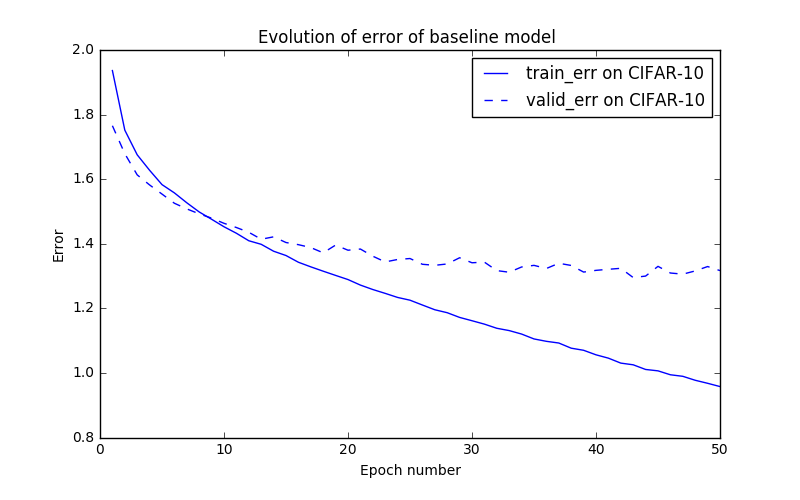
\includegraphics[width=3.3in]{baseline_error_cifar10}
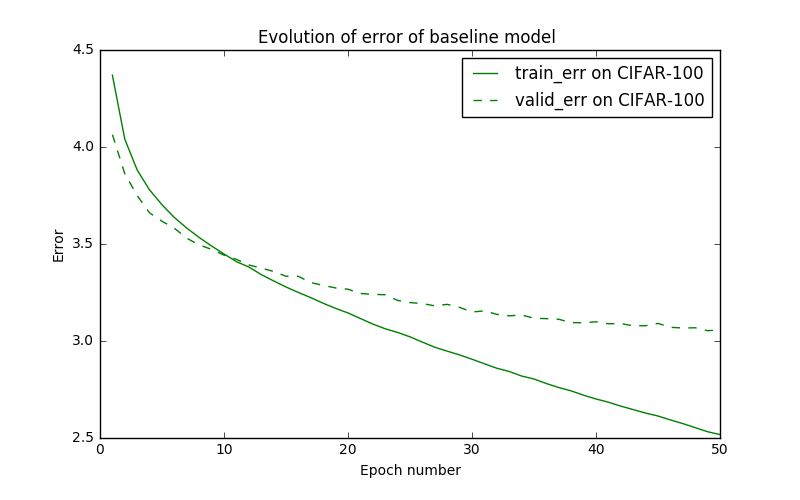
\includegraphics[width=3.3in]{baseline_error_cifar100}
\caption{Evolution of Error of baseline model on CIFAR-10(blue line) and CIFAR-100(green line) }
\end{center}
\end{figure}

\begin{table}[ht]
\centering 
\caption{Recognition statistic of baseline model}
\begin{tabular}{c c c c}
\toprule
Dateset & Final valid Acc.(\%) & Final valid Err.(loss) & Average training time\\
\midrule
CIFAR-10 & 0.54 & 1.32 & 28.56 \\
CIFAR-100 & 0.26 & 3.05 & 29.23  \\
\bottomrule
\end{tabular}
\end{table} 


Our further experiment will be built on the basis of this model. The problem contained in this model is that the model isn't complex enough to provide higher accuracy and it still has the trend to overfit. Our experiments will try to solve these problems. Also, the results(shown in Table 1) of this model will be the comparable result to evaluate our experiments result.
\section{Data augmentation}
\subsection{Motivation and methods}
Data augmentation is an effective method to reduce overfitting. It is widely used in today's deep neural network. The main idea of data augmentation is to enlarge the dataset using label-preserving transformation artificially (Krizhevsky, 2012). Through error evolution of baseline model, we could still find that the model has the trend to overfit. To avoid this, we implement two kinds of data augmentation methods according to several papers:

\begin{itemize}
\item First method is a random rotation method. This method only randomly rotate the image(by $\pm 90$\textdegree) and it has already been implemented in $Tensorflow$.
\item Second method is referring to He's(2016) work, their augmentation method includes padding the image to $36 \times 36$ dimension, then randomly flipping the image left to right, and finally randomly cropping the image down to $32 \times 32$ dimension.
\end{itemize}

Comparing with first method, second method is more complex because it does not only flipping but also transposition(padding and randomly cropping does this operation). In this section, we want to compare these two methods to see if they could help to reduce overfitting.

For the implementation, we build a $data\_augmentation()$ function to handle the source images and use $tf.map\_fn()$ in the function to apply transformation to each image in each batch. As for the first augmentation method, $tf.image.rot90()$ will be used to do rotation operation. And in implementation of the second method, we use $resize\_image\_with\_crop\_or\_pad()$ function to pad the image, $tf.image.random\_flip\_left\_right()$ to randomly flip the image and finally we use $tf.image.crop\_to\_bounding\_box()$ to do the random cropping.
  
\subsection{Experiments and results}
We add the data augmentation part in front of the baseline NN network to randomly transform the input data.

\begin{figure}[!h]
\begin{center}
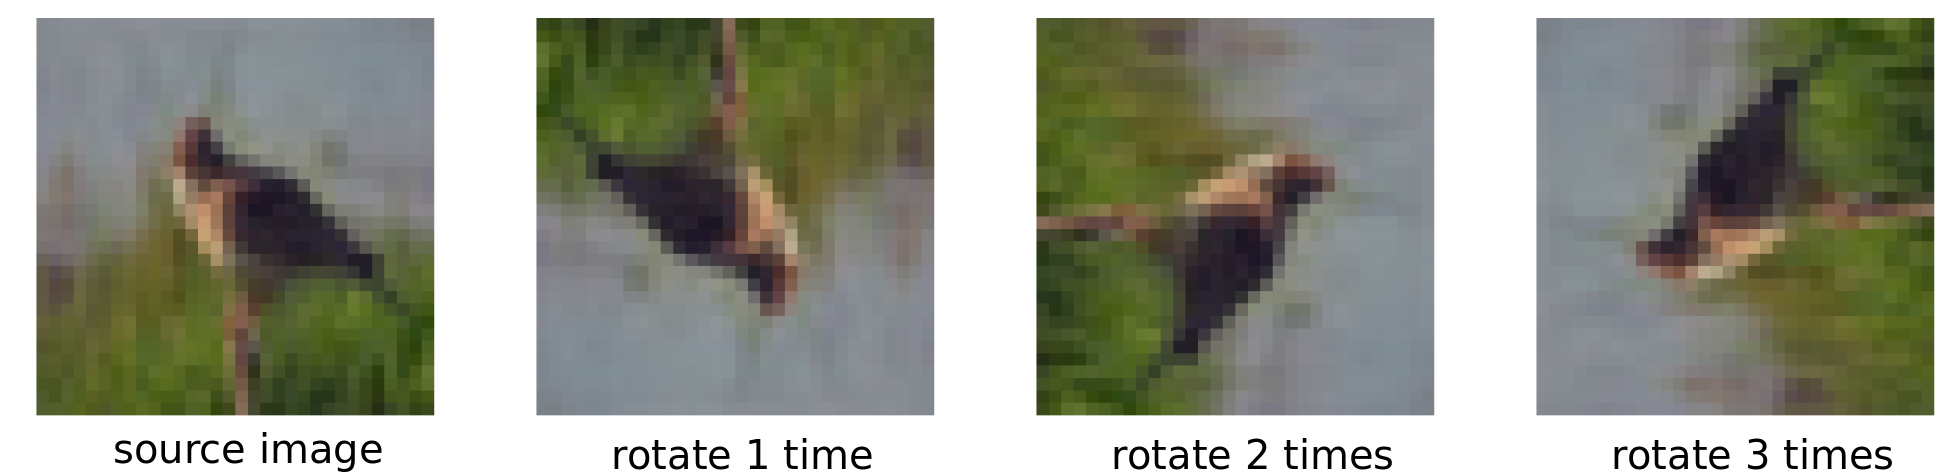
\includegraphics[width=5in]{rotate_plot}
\caption{Data augmentation(rotation method) steps and the transforming results}
\end{center}
\end{figure}

For the rotation method, the image will be randomly rotated by $90 $\textdegree several times and thus there will be 4 kinds of possible images with one input image. Besides the original images, the dataset is expanded threefold. The transforming results are shown below(Figure 2). 

As for the padding-flipping-cropping method, the transforming results are much more than the rotation method. There are 25 kinds of positions and 2 kinds of flipping directory, which means that the dataset is expanded 50 times potentially. The transforming results are shown below(Figure 3). From the results, the transformed image contains black border, which shows that the image is padded with black pixels and down cropped to $32\times 32$.

\begin{figure}[!h]
\begin{center}
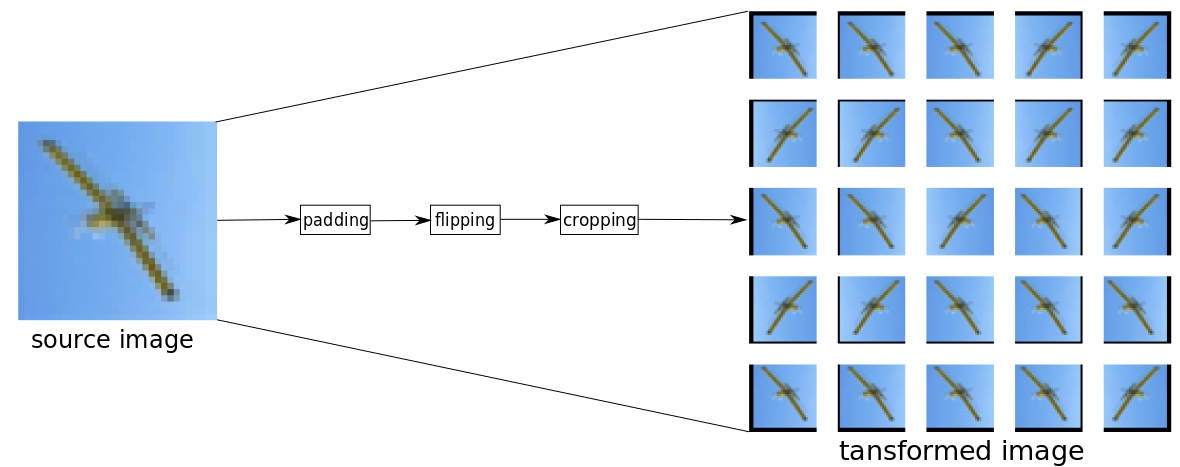
\includegraphics[width=5in]{aug_plot} 
\caption{Data augmentation(padding->flipping->cropping method) steps and the transforming results}
\end{center}
\end{figure}

We used both of these two methods to train our baseline model and the comparable evolution of accuracy and error is shown below (Figure 4). From the plot, we could find that the rotation method gives similar evolution to the baseline model in both training and validation process. The red solid curve shows that the padding-flipping-cropping method significantly slow down the learning process. As for the final result, these three models could achieve similar recognition result on validation set.

\begin{figure}[!h]
\begin{center}
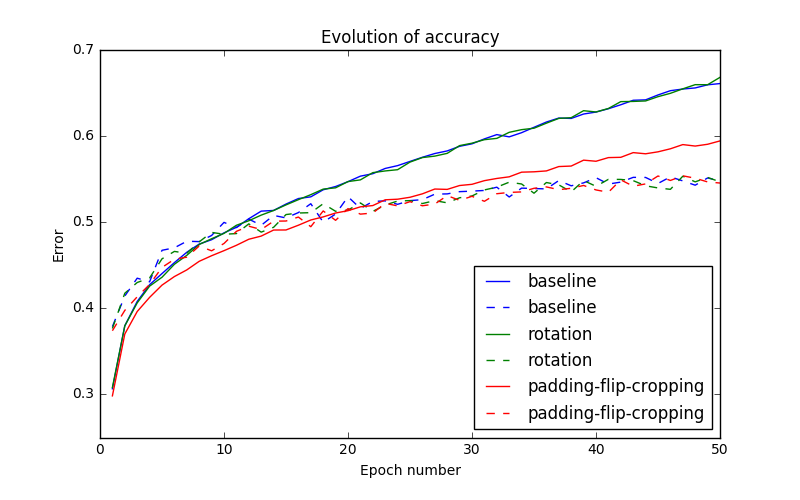
\includegraphics[width = 3.3in]{data_augmentation_acc}
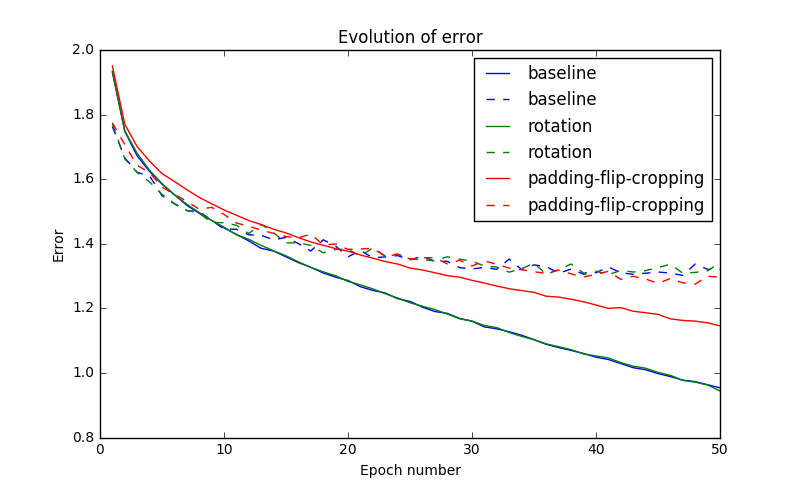
\includegraphics[width = 3.3in]{data_augmentation_err}
\caption{Evolution of accuracy(left) and error(right) of different data augmentation method (solid line shows the training evolution; dotted line shows the validation evolution)}
\end{center}
\end{figure}

We also record the training statistics for discussion. The final accuracy, loss and average training time is shown in Table 2. They all achieve the same validation accuracy and similar validation loss. 

\begin{table}[!h]
\centering 
\caption{Experiments design and results of data augmentation experiment}
\begin{tabular}{c c c c c}
\toprule
No. & Augmentation method & Final valid Acc.(\%) & Final valid Err.(loss) & Average training time(s)\\
\midrule
1 & Random rotation by 90\textdegree & 0.55 & 1.34 & 38.48 \\
2 & Padding-flipping-cropping & 0.55 & 1.30 & 38.81 \\
\bottomrule
\end{tabular}
\end{table}

\subsection{Conclusion and discussion}
From the experiments result we obtain above, it seems that the data augmentation doesn't provide any improvement to accuracy or loss. However, it truly influences the training process. We will discuss the results in two aspects: reducing overfitting and computational cost.

\textbf{Reducing Overfitting.} From the evolution plots, we find that the padding-flipping-cropping method significantly slow down the training curve from going higher while the rotation method provides a similar training curve comparing with the baseline model. It seems that the number of potential images determines the performance of data augmentation method. In our experiments, rotation method only provides 3 more kinds of potential images which makes no sense to the training process. On contrast, the padding-flipping-cropping method which gives 50 kinds of potential images could effectively reduce overfitting. Also, randomness should also be considered in designing augmentation strategy because it is obvious that too much randomness will finally make the system hard to converge. In the coming experiments, we will continue to use padding-flipping-cropping augmentation strategy to do data augmentation.

\textbf{Computational Cost.} By comparing the training time with baseline model(28.56s), the augmentation method takes much more time to do transforming operation. Fortunately, doing three operation (second method) doesn't take more time than only doing one operation (first method). The main cost of time comes from information transmission in $Tensorflow$. Hence, it's acceptable to apply data augmentation in further experiments.

In conclusion, padding-flipping-cropping method seems to be a better choice of augmentation strategy and we will use it to reduce overfitting.
 
\section{Convolutional neural network}
\subsection{Motivation and methods}
Convolutional neural network has been proven to achieve very good results in image recognition. It's definitely worth a trying in our experiments. However, to build a CNN model, there are many hyperparameters that need to be considered, which will make our experiments hard to design and carry out. In this experiment, we want to concentrate on kernel size in CNN to make a tighter focus. 

As for the implementation, we implement a $kernel$ function and $cnn\_layer$ function to build CNN. In $kernel$ function, we create the kernel weights and use L2 penalty as regularisation method. In $cnn\_layer$ function, we use $tf.nn.conv2d$ to calculate the convolution of input data and corresponding kernel. For the activation function, we set ReLU as default activation function in CNN layers.

Our architecture of CNN layer refers to He's(2016) work. The input data will first enter a convolutional layer with the kernel size of [3,3,3,64] (assume that the kernel size is $3\times 3\times 64$) and then follow with a max pooling layer to reduce the dimension by half. We will use $tf.nn.max\_pool$ to do the max pooling. After that, there will be another convolutional layer with the kernel size of [3,3,64,64]. In the end of the convolutional layers, a simple average pooling layer will be added to the architecture($tf.nn.avg\_pool$ could do this). Also, in each convolutional layer, batch normalisation(refer to coursework 3) will be used to the output of $cnn\_layer$. Finally, the output of convolutional layers will be passed to our baseline model to generate the final result. The entire architecture is shown below.

\begin{figure}[!ht]
\begin{center}
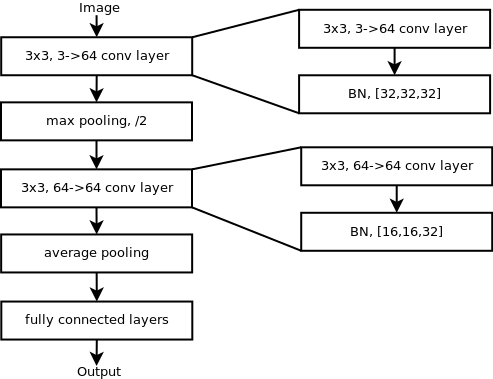
\includegraphics[width = 2in]{conv_diam_1}
\caption{Example architecture of experiment convolutional neural network}
\end{center}
\end{figure}

Kernel size would be the only hyperparameter we investigate in this experiment. He(2016) uses the kernel size of $3\times 3$ and the number of filters are $\{16,32,64\}$ in his deep network; Krizhevsky(2009) sets the kernel size to $5\times 5$ and the number of filters to $64$. Generally, the kernel size is always bigger than $2\times 2$ and smaller than $5\times 5$ and the filter number is usually either $32$ or $64$. So, we will test the kernel size of $3\times 3$ and $5\times 5$ and the filter number of $32$ and $64$.

\subsection{Experiments and results}
Follow He's(2016) experiments, we use Xavier initializer to initialize the kernel weights and set the weight decay of $0.0001$ and momentum of 0.9. Batch normalisation is applied to convolutional layers and dropout is applied to fully connected layers with the ratio of $0.8$ (refer to coursework 3). We start training with the learning rate of $0.01$ and manually divide it by 10 at 15th epoch and 30th epoch. The data augmentation method is padding-flipping-cropping method which we find it works well in previous experiments.

We compare kernel size of $\{3\times 3, 5\times 5 \}$ and the filter number of $\{32, 64\}$. The design of experiments and results are shown in Table 3. Experiment pair (1,3) and (2,4) could provide results to compare the performance of different kernel size. And experiment pair (1,2) and (3,4) could give the comparable result to evaluate the influence of filter number. 

\begin{table}[ht]
\centering 
\caption{Experiments design and results of kernel size experiment}
\begin{tabular}{c c c c c}
\toprule
No. & Kernel size & Final valid Acc.(\%) & Final valid Err.(loss) & Average training time(s)\\
\midrule
1 & $[3\times 3 \times 32]$ & 0.70 & 0.86 & 127.75  \\
2 & $[3\times 3 \times 64]$ & 0.71 & 0.89 & 251.30 \\
3 & $[5\times 5 \times 32]$ & 0.71 & 0.84 & 160.30 \\
4 & $[5\times 5 \times 64]$ & 0.72 & 0.84 & 332.83 \\
\bottomrule
\end{tabular}
\end{table}

From table 3, we find that these four kinds of kernel size achieves similar validation accuracy. However, their validation loss are different -- it seems that kernel size of $[5\times 5 \times 64]$ converges better than the others since it gets lower validation loss and higher accuracy. To evaluate the training process, we also plot the evolution of accuracy and loss(Figure 6).

\begin{figure}[!ht]
\begin{center}
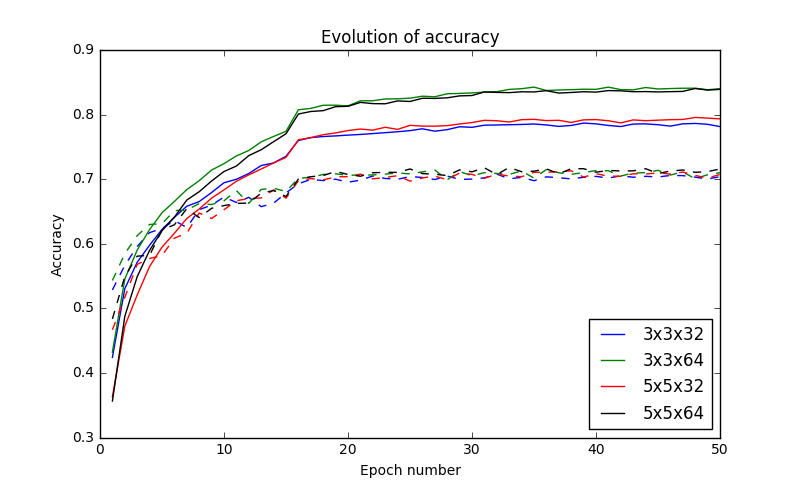
\includegraphics[width = 3.3in]{kernel_size_acc}
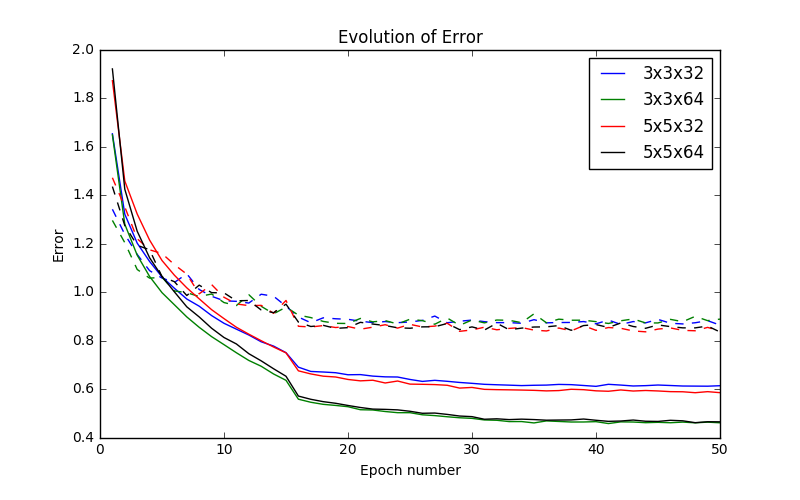
\includegraphics[width = 3.3in]{kernel_size_err}
\caption{Evolution of accuracy and loss of kernel size experiments. Solid line shows the training evolution and dotted shows the validation evolution}
\end{center}
\end{figure}

The evolution plot shows that different kernel size doesn't influence the result but filter number does. The training accuracy of 32 filter number is fluctuating at around 0.76 and that of 64 filter number is fluctuating at around 0.82. The training loss follows the similar trend -- same number of filters gives the same evolution of training loss and the loss of 32 filter number(around 0.60) is bigger than that of 64 filter number(around 0.48). As for the validation process, they share similar trend and generally, bigger filter number provides slightly higher accuracy and lower loss. 

\subsection{Conclusion and discussion}

\textbf{Number of filters.} From what is shown in evolution plots, we can indicate that a larger filter number could give higher training accuracy. But high training accuracy doesn't lead to high validation accuracy. I think we could explain this by regarding the CNN as a simple fully connected network -- increasing the number of filter is similar to expanding the width of a fully connected network. The wider width could provide a more complex model so that it could fit the training data effectively. Similarly, larger number of filters makes the model complex enough to give better result on training set. 

\textbf{Kernel size.} Convolutional neural network works based on three main assumption (Hechtlinger,2017):

\begin{enumerate}
\item \textbf{Local connectivity assumption:}
The signal in visual data tends to be highly correlated in
local regions, and mostly uncorrelated in global regions.

\item \textbf{Shared weights assumption:}
The same convolution is globally valid across the image,
resulting in a significant parameter reduction.

\item \textbf{Grid structure of the image:}
Enabling a straight forward re-scaling of the feature layers
through the process of max pooling.
\end{enumerate}

From above assumption, the low level feature we generated from the convolutional kernel is highly depend on how strongly a feature is correlated to its neighbours. And the kernel size should be determined by the relevance between feature and its local region. Kernel size of $3 \times 3$ means the feature is slightly correlated to its neighbour pixels and the kernel size of $5 \time 5$ means the relevance is stronger. In our experiments, $3 \times 3$ and $5 \times 5$ provides similar results, which means that they could all extracted the low level features for the requirement of recognition. Hence, if we take into account the problem of computational cost, it's a good choice to choose the kernel size of $3\times 3\times 64$ for further experiments. 

\section{Mini residual neural network and further attempt}
\subsection{Motivation and methods}
Residual learning method is proposed to prevent the problem of degradation which indicates that the recognition accuracy gets saturated and then degrades rapidly with the depth of network increasing. The degradation problem makes the neural network hard to optimize -- we could also find this phenomenon in our follow experiments.

The main idea of residual learning method is to reformulate the optimal function. Assume that the original function $F(x)$ is a linear function with nonlinearity activation function. It could be defined like this:

\begin{equation}
	F(x) = \sigma(x,W)
\end{equation}

Where $W$ is the weights parameter and $\sigma$ refers to the activation function (usually ReLU in this experiment). This formulation comes from a hypothesis that multiple nonlinear layers can asymptotically approximate complicated target function $T(x)$  (Montufar,2014). Hence, it is also the same that the multiple nonlinear layers could approximate the residual function $T(x)-x$. The optimal function is then reformulated to $F(x) + x := T(x)$. Our new prediction function is like this:

\begin{equation}
	F'(x) = \sigma(x,W) + x_l
\end{equation}

In the formulation, $x_l$ refers to the output of previous layer and in this case, $\sigma$ might represent a few stacked layers.  The implementation of residual could be done by adding shortcut connection from previous layer to the current output. Normally, the shortcut connection spans two or three layers of neural network because skipping only one layer doesn't provide any improvement in He's(2016) experiments. The structure of a residual unit is shown in Figure 7.

\begin{figure}[!h]
\begin{center}
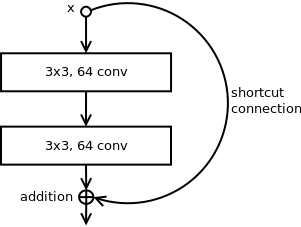
\includegraphics[width = 1.5in]{residualunit}
\caption{Residual unit structure}
\end{center}
\end{figure}

There are several ways to define $\sigma$. According He(2016), the $\sigma$ function includes the pre-activation function and the post-activation function(the normal one in common neural network). Pre-activation function puts activation function before weight for the reason that activation function could be applied to previous input. The structure of post-(Figure 8.(a)) and pre-activation(Figure 8.(b)) function are shown below.

\begin{figure}[!h]
\begin{center}
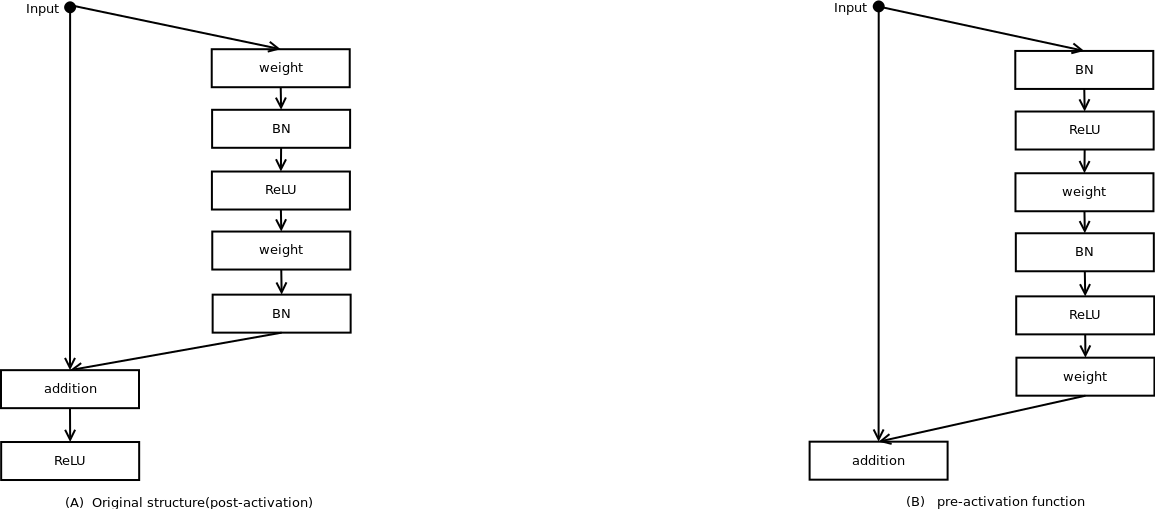
\includegraphics[width = 4in]{res_activation_function}
\caption{$\sigma$ function definition}
\end{center}
\end{figure}

In this experiment, we will use pre-activation method to build our residual neural network because it has been proven to give better results in deep residual network(He,2016).

As for the implementation part, we create a $residual\_layer$ function to build residual units. The function receives the output from the upper layer and the output from two layers before the current layer. Then, the batch normalisation we implemented last time and ReLU will also be applied to residual unit.

\subsection{Experiments and results}

To compare the performance of residual neural network, we design two groups of experiments. The first group is about the non-residual convolutional neural network with different depth of architecture to provide a comparable result. Second group is to apply residual learning method to the above model. So, by comparing the result of these two group of experiments, we could investigate the performance of residual learning method in shallow convolution neural network.

We first restructure the convolutional layer in CNN experiments to the form of pre-activation function. Then, we add another convolutional layer to the model in order to make the architecture deep enough to apply residual learning method. The architecture of new CNN model is shown in Figure 9.(a).

\begin{figure}[!h]
\begin{center}
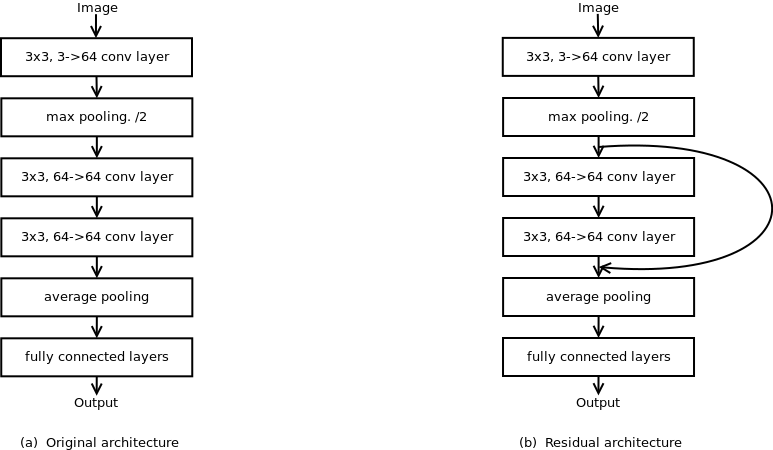
\includegraphics[width = 4in]{residual_architecture}
\caption{New CNN architecture(left) and ResNN architecture(right)}
\end{center}
\end{figure}

The architecture of residual neural network is shown in Figure 9.(b). From the diagram, we only add the shortcut connection to the central convolutional layers because they have the same dimension so that we don't need to add weights to change the dimension. Our experiments setting follows the setting of CNN experiments, the kernel weights are initialized by Xavier initializer and applied weight decay of 0.0001 and momentum of 0.9. The start learning rate is 0.01 and it will be divided by 10 at 15th epoch and 30th epoch. The data augmentation strategy follows what we have got from data augmentation experiments. For further experiments, we also test the architecture of 5 and 7 convolutional layers. Our experiments design and results are shown in Table 4. Because we run experiments 1.3 and 2.3 on $msccluster$, the training time is highly related to computing context that we don't record the training time.

\begin{table}[ht]
\centering 
\caption{Experiments design and results of ResNN experiment}
\begin{tabular}{c l c c c}
\toprule
No. & Architecture & Final valid Acc.(\%) & Final valid Err.(loss) & Average training time(s)\\
\midrule
1.1 & 3 conv layers & 0.74 & 0.80 & 338.08 \\
1.2 & 5 conv layers & 0.75 & 0.76 & 457.23 \\
1.3 & 7 conv layers & 0.73 & 0.81 & --  \\
\midrule
2.1 & 3 conv layers with residual & 0.72 & 0.88 & 342.18 \\
2.2 & 5 conv layers with residual & 0.73 & 0.79 & 452.56 \\
2.3 & 7 conv layers with residual & 0.75 & 0.75 & --  \\
\bottomrule
\end{tabular}
\end{table}

For evaluating the training process, we also plot the evolution of accuracy and loss of training set and validation set. The plots are shown in Figure 10. 

\begin{figure}[!h]
\begin{center}
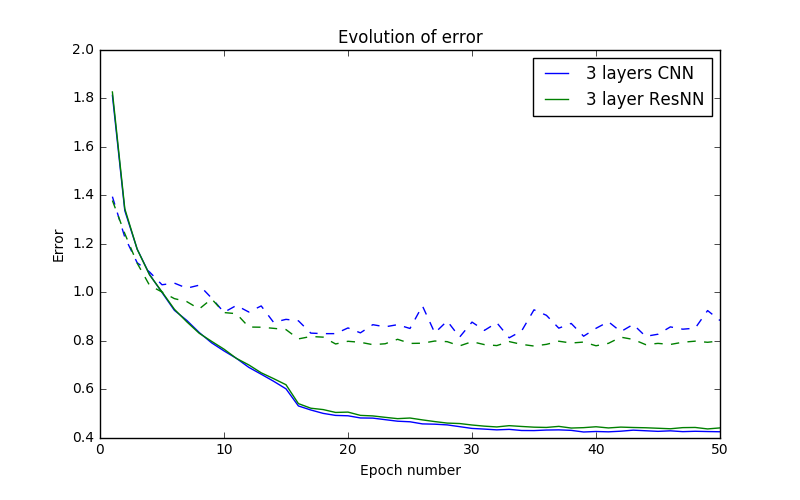
\includegraphics[width = 3.3in]{res_3layers_err}
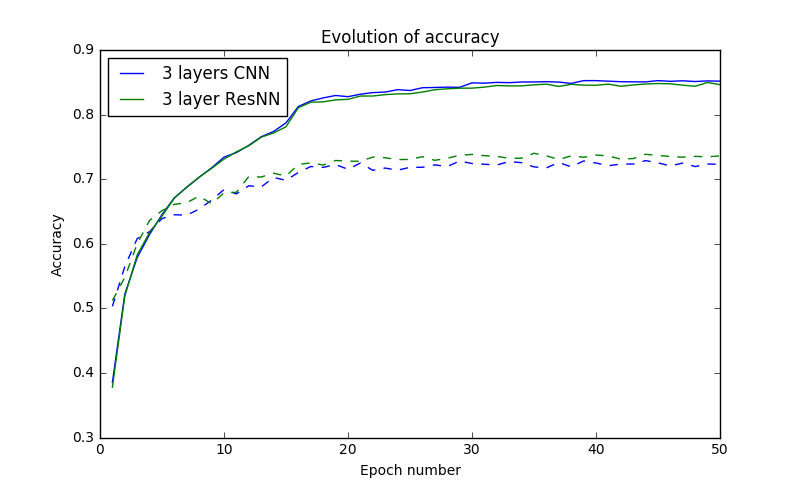
\includegraphics[width = 3.3in]{res_3layers_acc}
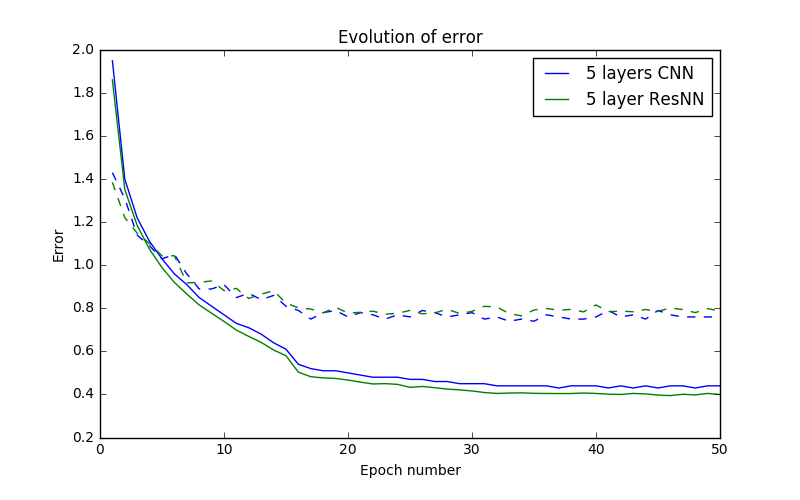
\includegraphics[width = 3.3in]{res_5layers_err}
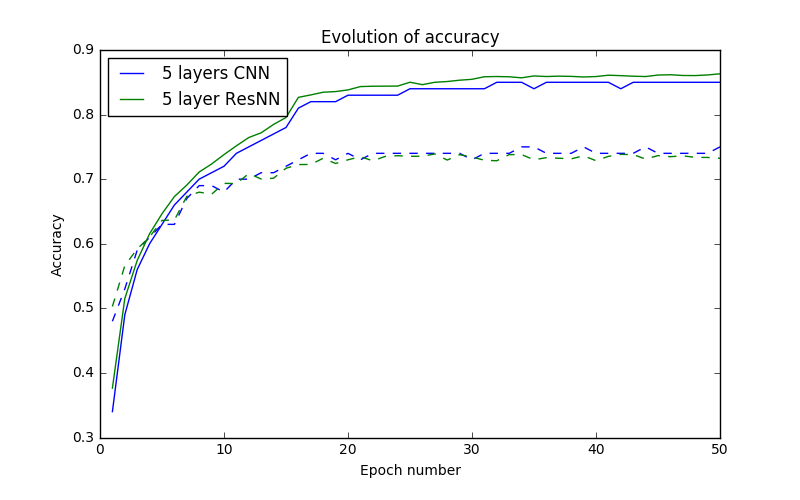
\includegraphics[width = 3.3in]{res_5layers_acc}
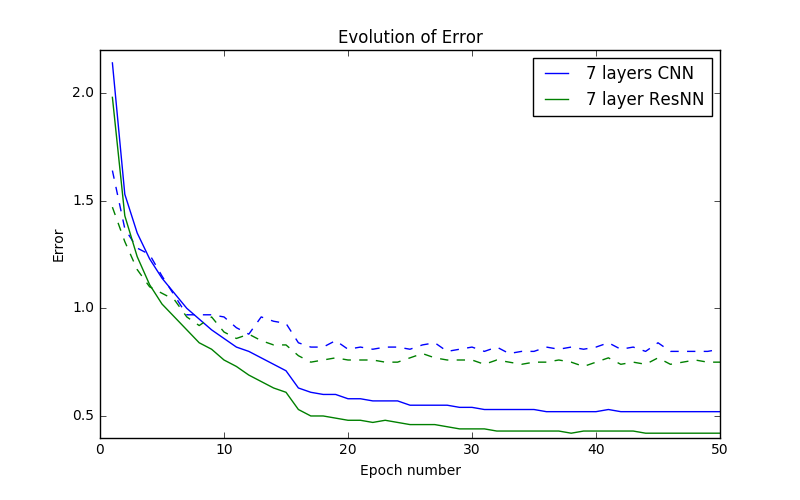
\includegraphics[width = 3.3in]{res_7layers_err}
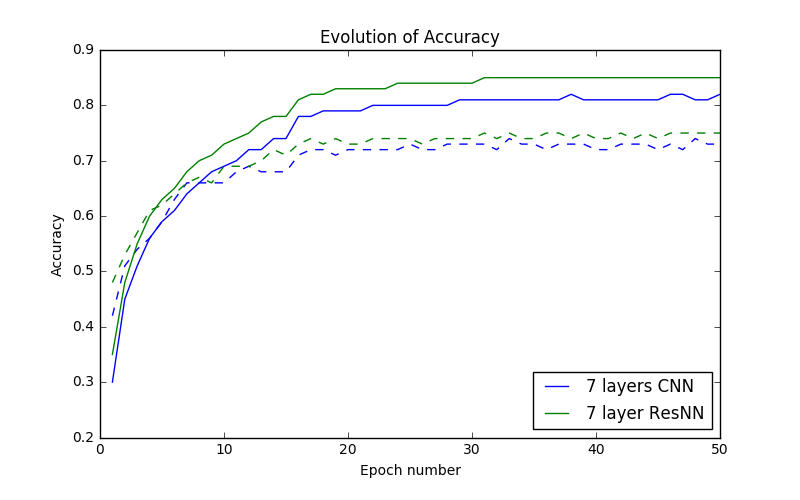
\includegraphics[width = 3.3in]{res_7layers_acc}
\caption{Evolution of error(left) and accuracy(right) on training set and validation set. Solid line refers to the training process and dotted line refers to validation process.}
\end{center}
\end{figure}

From the plots, we can investigate that the distance between training curve of CNN and ResNN becomes larger with the increase of convolutional layers. Also, combining with the table statistics, with the increase of convolutional layers, the performance of ResNN continues becoming better and the performance of CNN gets stable, even worse.  

\subsection{Conclusion and discussion} 

What we have observed about convolutional network meets the degradation problem which leads recognition accuracy get saturated and makes the network hard to optimize. In detail, in our experiments, adding more layers to the network can lead to optimization problems(see experiments group 1), which do not allow the network to learn as well as a shallower network could. By comparing the results of ResNN, we could find that residual learning method gives network the ability to continue to converge and generate better results.

In our experiments, the results show that residual learning method also effectively reduces degradation problem and improves the performance in shallow networks. He(2016) explains why residual learning method could provide this kind of ability -- if the optimal function is closer to an identity mapping than to a zero mapping, it should be easier for the solver to find the perturbations with reference to an identity mapping, than to learn the function as a new one. In another word, it is easier for the network to learn $F(x) = 0$ than $F(x) = x$. Hence, if we add a small residual to optimal function, the network will start to learn $F(x) = 0$ so that the network could enjoy the superior performance provided by a deeper network.

In conclusion, residual neural network seems to be the most satisfied model we obtained for the reason that it could generate good result even in deeper neural networks. We finally apply this model to CIFAR-100 dataset to test if it could get good results as well as on CIFAR-10. The recognition results and evolution plots are shown below(Table 5 and Figure 11):

\begin{table}[ht]
\centering 
\caption{Recognition statistic of baseline model \& satisfied model}
\begin{tabular}{c c c c}
\toprule
Dateset & Model & Final valid Acc.(\%) & Final valid Err.(loss)\\
\midrule
\multirow{2}{*}{CIFAR-10} & baseline & 0.54 & 1.32 \\
 & ResNN & \textbf{0.75} & \textbf{0.75}  \\
\midrule
\multirow{2}{*}{CIFAR-100} & baseline & 0.26 & 3.05   \\
 & ResNN & \textbf{0.39} & \textbf{2.89}   \\
\bottomrule
\end{tabular}
\end{table} 

\begin{figure}[!h]
\begin{center}
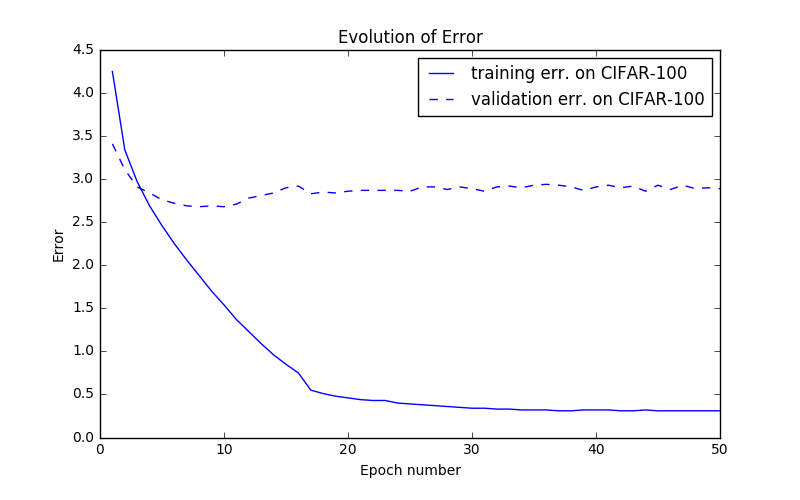
\includegraphics[width = 3.3in]{cifar100_err}
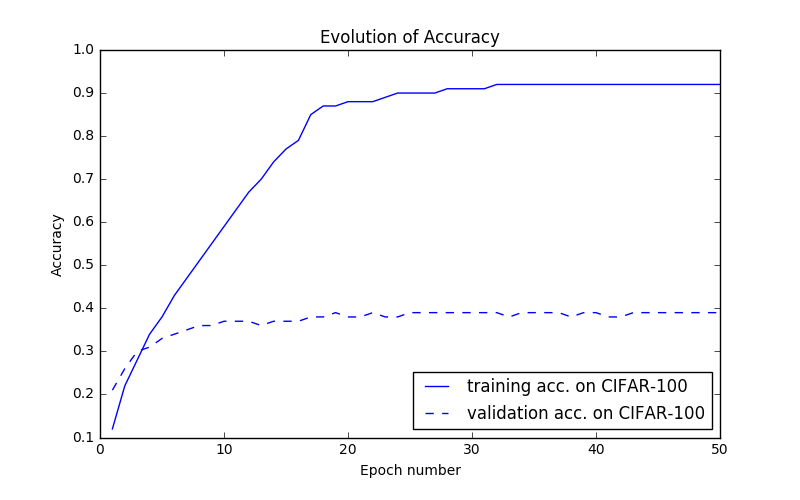
\includegraphics[width = 3.3in]{cifar100_acc}
\caption{Evolution of error(left) and accuracy(right) on CIFAR-100. Solid line refers to the training process and dotted line refers to validation process.}
\end{center}
\end{figure}

The plots and statistics show that ResNN could achieve good result on CIFAR-100 as well as on CIFAR-10. Also, the recognition accuracy on CIFAR-100 still seems not satisfactory. This also indicates that there are many aspects in our model that need to be improved. 

\section{Conclusion}
In this experiment, we first test different kinds of data augmentation methods and find that padding-flipping-cropping method could effectively prevent overfitting with acceptable computational cost. Then, we move on to convolutional neural network to build a suitable network for further exploration. In the CNN experiment, we apply different kernel size and finally find a suitable kernel size for building residual neural network. Finally, we apply residual learning method to the model we get in CNN experiments and find that residual learning method could also effectively reduce the degradation problem.

With all these experiments, we finally build the most satisfying model. By comparing with the baseline model, our model could significantly improve the performance of recognition system.

For further work, I think one possible direction is to adjust the residual of residual neural network to fit the model. In our experiment, we only try simple identify mapping. However, according to He(2016), the residual function could also be learned to adapt the model. Another possible direction might be expanding the model to more complex dataset(eg. ImageNet). Although the colors and textures in the images of CIFAR-10/CIFAR-100 varies greatly, the images themselves are not big enough to contain more noise which will cause obstacles in recognition process. Hence, for further prove of our conclusion, we need to apply our model to different dataset to test its performance. 
\newpage
\begin{thebibliography}{9}
\bibitem{he2015}
  He, Kaiming, et al.
  "Deep residual learning for image recognition."
  \emph{Proceedings of the IEEE Conference on Computer Vision and Pattern Recognition.}
  2016.
\bibitem{he2016}
  He, Kaiming, et al.
  "Identity mappings in deep residual networks."
  \emph{European Conference on Computer Vision. Springer International Publishing,}
  2016.
\bibitem{krizhevsky2009}
  Krizhevsky, Alex, and Geoffrey Hinton
  "Learning multiple layers of features from tiny images."
  (2009).  
\bibitem{veit2016}
  Veit, Andreas, Michael J. Wilber, and Serge Belongie.
  "Residual networks behave like ensembles of relatively shallow networks."
  \emph{Advances in Neural Information Processing Systems.}
  2016.
\bibitem{lee2015}
  Lee, Chen-Yu, et al.
  "Deeply-Supervised Nets."
  \emph{AISTATS.}
  Vol. 2. No. 3. 2015.
\bibitem{ciregan2012}
  Ciregan, Dan, Ueli Meier, and Jürgen Schmidhuber.
  "Multi-column deep neural networks for image classification."
  \emph{Computer Vision and Pattern Recognition (CVPR), 2012 IEEE Conference on.}
  IEEE, 2012.
\bibitem{Krizhevsky2012}
  Krizhevsky, Alex, Ilya Sutskever, and Geoffrey E. Hinton.
  "Imagenet classification with deep convolutional neural networks."
  \emph{Advances in neural information processing systems.}
  2012.
\bibitem{ciresan2012}
  Ciresan, Dan C., et al.
  "High-performance neural networks for visual object classification."
  \emph{arXiv preprint arXiv:1102.0183}
  (2011).
\bibitem{montufar2014}
  Montufar, Guido F., et al.
  "On the number of linear regions of deep neural networks."
  \emph{Advances in neural information processing systems.}
  2014.  
\bibitem{cs231n}
  CS231n.
  Convolutional Neural Networks for Visual Recognition.
  \emph{http://cs231n.github.io/convolutional-networks/\#add .}
  2016.   
\bibitem{hechtlinger2017}
  Yotam Hechtlinger, Purvasha Chakravarti and Jining Qin.
  "Convolutional neural networks generalization utilizing the data graph structure."
  \emph{ICLR.}
  2017.
\bibitem{cw2}
  s1626868.
  "Baseline experiments on CIFAR-10 and CIFAR-100."
  \emph{MLP coursework report}
  2017.

\end{thebibliography}

\end{document}